% Options for packages loaded elsewhere
\PassOptionsToPackage{unicode}{hyperref}
\PassOptionsToPackage{hyphens}{url}
\PassOptionsToPackage{dvipsnames,svgnames*,x11names*}{xcolor}
%
\documentclass[
]{article}
\usepackage{lmodern}
\usepackage{amssymb,amsmath,siunitx}
\usepackage{ifxetex,ifluatex}
\ifnum 0\ifxetex 1\fi\ifluatex 1\fi=0 % if pdftex
  \usepackage[T1]{fontenc}
  \usepackage[utf8]{inputenc}
  \usepackage{textcomp} % provide euro and other symbols
\else % if luatex or xetex
  \usepackage{unicode-math}
  \defaultfontfeatures{Scale=MatchLowercase}
  \defaultfontfeatures[\rmfamily]{Ligatures=TeX,Scale=1}
  \setmainfont[]{cochineal}
  \setsansfont[]{Fira Sans}
\fi
% Use upquote if available, for straight quotes in verbatim environments
\IfFileExists{upquote.sty}{\usepackage{upquote}}{}
\IfFileExists{microtype.sty}{% use microtype if available
  \usepackage[]{microtype}
  \UseMicrotypeSet[protrusion]{basicmath} % disable protrusion for tt fonts
}{}
\makeatletter
\@ifundefined{KOMAClassName}{% if non-KOMA class
  \IfFileExists{parskip.sty}{%
    \usepackage{parskip}
  }{% else
    \setlength{\parindent}{0pt}
    \setlength{\parskip}{6pt plus 2pt minus 1pt}}
}{% if KOMA class
  \KOMAoptions{parskip=half}}
\makeatother
\usepackage{xcolor}
\IfFileExists{xurl.sty}{\usepackage{xurl}}{} % add URL line breaks if available
\IfFileExists{bookmark.sty}{\usepackage{bookmark}}{\usepackage{hyperref}}
\hypersetup{
  pdftitle={Data Science for Economists},
  colorlinks=true,
  linkcolor=Maroon,
  filecolor=Maroon,
  citecolor=Blue,
  urlcolor=blue,
  pdfcreator={LaTeX via pandoc}}
\urlstyle{same} % disable monospaced font for URLs
\usepackage[margin=1in]{geometry}
\usepackage{color}
\usepackage{fancyvrb}
\newcommand{\VerbBar}{|}
\newcommand{\VERB}{\Verb[commandchars=\\\{\}]}
\DefineVerbatimEnvironment{Highlighting}{Verbatim}{commandchars=\\\{\}}
% Add ',fontsize=\small' for more characters per line
\usepackage{framed}
\definecolor{shadecolor}{RGB}{248,248,248}
\newenvironment{Shaded}{\begin{snugshade}}{\end{snugshade}}
\newcommand{\AlertTok}[1]{\textcolor[rgb]{0.94,0.16,0.16}{#1}}
\newcommand{\AnnotationTok}[1]{\textcolor[rgb]{0.56,0.35,0.01}{\textbf{\textit{#1}}}}
\newcommand{\AttributeTok}[1]{\textcolor[rgb]{0.13,0.29,0.53}{#1}}
\newcommand{\BaseNTok}[1]{\textcolor[rgb]{0.00,0.00,0.81}{#1}}
\newcommand{\BuiltInTok}[1]{#1}
\newcommand{\CharTok}[1]{\textcolor[rgb]{0.31,0.60,0.02}{#1}}
\newcommand{\CommentTok}[1]{\textcolor[rgb]{0.56,0.35,0.01}{\textit{#1}}}
\newcommand{\CommentVarTok}[1]{\textcolor[rgb]{0.56,0.35,0.01}{\textbf{\textit{#1}}}}
\newcommand{\ConstantTok}[1]{\textcolor[rgb]{0.56,0.35,0.01}{#1}}
\newcommand{\ControlFlowTok}[1]{\textcolor[rgb]{0.13,0.29,0.53}{\textbf{#1}}}
\newcommand{\DataTypeTok}[1]{\textcolor[rgb]{0.13,0.29,0.53}{#1}}
\newcommand{\DecValTok}[1]{\textcolor[rgb]{0.00,0.00,0.81}{#1}}
\newcommand{\DocumentationTok}[1]{\textcolor[rgb]{0.56,0.35,0.01}{\textbf{\textit{#1}}}}
\newcommand{\ErrorTok}[1]{\textcolor[rgb]{0.64,0.00,0.00}{\textbf{#1}}}
\newcommand{\ExtensionTok}[1]{#1}
\newcommand{\FloatTok}[1]{\textcolor[rgb]{0.00,0.00,0.81}{#1}}
\newcommand{\FunctionTok}[1]{\textcolor[rgb]{0.13,0.29,0.53}{\textbf{#1}}}
\newcommand{\ImportTok}[1]{#1}
\newcommand{\InformationTok}[1]{\textcolor[rgb]{0.56,0.35,0.01}{\textbf{\textit{#1}}}}
\newcommand{\KeywordTok}[1]{\textcolor[rgb]{0.13,0.29,0.53}{\textbf{#1}}}
\newcommand{\NormalTok}[1]{#1}
\newcommand{\OperatorTok}[1]{\textcolor[rgb]{0.81,0.36,0.00}{\textbf{#1}}}
\newcommand{\OtherTok}[1]{\textcolor[rgb]{0.56,0.35,0.01}{#1}}
\newcommand{\PreprocessorTok}[1]{\textcolor[rgb]{0.56,0.35,0.01}{\textit{#1}}}
\newcommand{\RegionMarkerTok}[1]{#1}
\newcommand{\SpecialCharTok}[1]{\textcolor[rgb]{0.81,0.36,0.00}{\textbf{#1}}}
\newcommand{\SpecialStringTok}[1]{\textcolor[rgb]{0.31,0.60,0.02}{#1}}
\newcommand{\StringTok}[1]{\textcolor[rgb]{0.31,0.60,0.02}{#1}}
\newcommand{\VariableTok}[1]{\textcolor[rgb]{0.00,0.00,0.00}{#1}}
\newcommand{\VerbatimStringTok}[1]{\textcolor[rgb]{0.31,0.60,0.02}{#1}}
\newcommand{\WarningTok}[1]{\textcolor[rgb]{0.56,0.35,0.01}{\textbf{\textit{#1}}}}
\usepackage{graphicx}
\makeatletter
\def\maxwidth{\ifdim\Gin@nat@width>\linewidth\linewidth\else\Gin@nat@width\fi}
\def\maxheight{\ifdim\Gin@nat@height>\textheight\textheight\else\Gin@nat@height\fi}
\makeatother
% Scale images if necessary, so that they will not overflow the page
% margins by default, and it is still possible to overwrite the defaults
% using explicit options in \includegraphics[width, height, ...]{}
\setkeys{Gin}{width=\maxwidth,height=\maxheight,keepaspectratio}
% Set default figure placement to htbp
\makeatletter
\def\fps@figure{htbp}
\makeatother
\setlength{\emergencystretch}{3em} % prevent overfull lines
\providecommand{\tightlist}{%
  \setlength{\itemsep}{0pt}\setlength{\parskip}{0pt}}
\setcounter{secnumdepth}{-\maxdimen} % remove section numbering
%% See: https://bookdown.org/yihui/rmarkdown-cookbook/multi-column.html
%% I've made some additional adjustments based on my own preferences (e.g. cols
%% should be top-aligned in case of uneven vertical length)
\newenvironment{columns}[1][]{}{}

\newenvironment{column}[1]{\begin{minipage}[t]{#1}\ignorespaces}{%
\end{minipage}
\ifhmode\unskip\fi
\aftergroup\useignorespacesandallpars
}

\def\useignorespacesandallpars#1\ignorespaces\fi{%
#1\fi\ignorespacesandallpars}

\makeatletter
\def\ignorespacesandallpars{%
  \@ifnextchar\par
    {\expandafter\ignorespacesandallpars\@gobble}%
    {}%
}
\makeatother
\usepackage{float}
\usepackage{booktabs}
\usepackage{longtable}

\title{Data Science for Economists}
\usepackage{etoolbox}
\makeatletter
\providecommand{\subtitle}[1]{% add subtitle to \maketitle
  \apptocmd{\@title}{\par {\large #1 \par}}{}{}
}
\makeatother
\subtitle{Lecture 8: Regression analysis in R}
\usepackage{authblk}
                                        \author[]{Grant R. McDermott}
                                                            \affil{University
of Oregon \textbar{} \href{https://github.com/uo-ec607/lectures}{EC
607}}
                                            \date{}

\begin{document}
\maketitle

{
\hypersetup{linkcolor=}
\setcounter{tocdepth}{2}
\tableofcontents
}
Today's lecture explores

\hypertarget{software-requirements}{%
\subsection{Software requirements}\label{software-requirements}}

\hypertarget{r-packages}{%
\subsubsection{R packages}\label{r-packages}}

It's important to note that ``base'' R already provides all of the tools
to implement a fixed effects regression, \textbf{but} you'll quickly hit
walls due to memory caps. Instead, I want to introduce \textbf{fixest},
short for Fixed-Effects Estimation, which provides lightning fast fixed
effects estimation and make your life much easier.

\begin{itemize}
\tightlist
\item
  New: \textbf{fixest}, \textbf{wooldridge}
\item
  Already used: \textbf{tidyverse}, \textbf{hrbrthemes},
  \textbf{listviewer}, \textbf{estimatr}, \textbf{ivreg},
  \textbf{sandwich}, \textbf{lmtest}, \textbf{mfx}, \textbf{margins},
  \textbf{broom}, \textbf{modelsummary}, \textbf{vtable},
  \textbf{rstanarm}
\end{itemize}

A convenient way to install (if necessary) and load everything is by
running the below code chunk.

\begin{Shaded}
\begin{Highlighting}[]
\DocumentationTok{\#\# Load and install the packages that we\textquotesingle{}ll be using today}
\ControlFlowTok{if}\NormalTok{ (}\SpecialCharTok{!}\FunctionTok{require}\NormalTok{(}\StringTok{"pacman"}\NormalTok{)) }\FunctionTok{install.packages}\NormalTok{(}\StringTok{"pacman"}\NormalTok{)}
\NormalTok{pacman}\SpecialCharTok{::}\FunctionTok{p\_load}\NormalTok{(mfx, tidyverse, hrbrthemes, estimatr, ivreg, fixest, sandwich, wooldridge,}
\NormalTok{               lmtest, margins, vtable, broom, modelsummary)}

\DocumentationTok{\#\# My preferred ggplot2 plotting theme (optional)}
\FunctionTok{theme\_set}\NormalTok{(}\FunctionTok{theme\_minimal}\NormalTok{())}
\end{Highlighting}
\end{Shaded}

\hypertarget{note-on-fixest-and-feols}{%
\paragraph{Note on fixest and feols}\label{note-on-fixest-and-feols}}

I'll be using fixest and feols throughout these notes. The fixest
package is a new package that is very fast and has a lot of
functionality. It has several bits of funtionality like \texttt{feols()}
and \texttt{etable()}, which are powerful functions for making
regressions and putting the output into tables that work well together.
\texttt{feols()} works very much like \texttt{lm()} in base R, but with
a few added bonuses.

\hypertarget{panel-models}{%
\subsubsection{Panel models}\label{panel-models}}

A panel dataset is one in which we view a single unit over multiple
periods of time, so a balanced panel has the same number of observations
for each unit. For example, we might have data on 100 countries over 10
years, or 50 US states over 20 years. We can then take unit fixed
effects, which lets us compare between years within a single unit.
Similarly, we can take time fixed effects to compare between units
within a given point in time. If our dataset has other dimensions that
vary in a way that is not collinear with unit or time, we can also take
a fixed effect for that -- though again, you want to be careful about
throwing in fixed effects.

\hypertarget{dataset}{%
\subsection{Dataset}\label{dataset}}

Let me introduce the dataset we'll be using, \texttt{crime4}. It comes
from Jeffrey Wooldridge's R package -- Dr.~Wooldridge is one of the most
accomplished professors of econometrics on the planet. I was tipped off
about his package by Nick Huntington-Klein's own
\href{https://github.com/NickCH-K/EconometricsSlides}{lecture notes.}.
The dataset shows county probability of arrest and county crime rate by
year.

\begin{Shaded}
\begin{Highlighting}[]
\FunctionTok{data}\NormalTok{(crime4)}
\NormalTok{crime4 }\SpecialCharTok{\%\textgreater{}\%}
  \FunctionTok{select}\NormalTok{(county, year, crmrte, prbarr) }\SpecialCharTok{\%\textgreater{}\%}
  \FunctionTok{rename}\NormalTok{(}\AttributeTok{County =}\NormalTok{ county,}
         \AttributeTok{Year =}\NormalTok{ year,}
         \AttributeTok{CrimeRate =}\NormalTok{ crmrte,}
         \AttributeTok{ProbofArrest =}\NormalTok{ prbarr) }\SpecialCharTok{\%\textgreater{}\%}
  \FunctionTok{slice}\NormalTok{(}\DecValTok{1}\SpecialCharTok{:}\DecValTok{9}\NormalTok{) }\SpecialCharTok{\%\textgreater{}\%}
\NormalTok{  knitr}\SpecialCharTok{::}\FunctionTok{kable}\NormalTok{(}\AttributeTok{note =} \StringTok{\textquotesingle{}...\textquotesingle{}}\NormalTok{) }\SpecialCharTok{\%\textgreater{}\%}
\NormalTok{  kableExtra}\SpecialCharTok{::}\FunctionTok{add\_footnote}\NormalTok{(}\StringTok{\textquotesingle{}9 rows out of 630. "Prob. of Arrest" is estimated probability of being arrested when you commit a crime\textquotesingle{}}\NormalTok{, }\AttributeTok{notation =} \StringTok{\textquotesingle{}none\textquotesingle{}}\NormalTok{)}
\end{Highlighting}
\end{Shaded}

County

Year

CrimeRate

ProbofArrest

1

81

0.0398849

0.289696

1

82

0.0383449

0.338111

1

83

0.0303048

0.330449

1

84

0.0347259

0.362525

1

85

0.0365730

0.325395

1

86

0.0347524

0.326062

1

87

0.0356036

0.298270

3

81

0.0163921

0.202899

3

82

0.0190651

0.162218

3

83

0.0151492

0.181586

3

84

0.0136621

0.194986

3

85

0.0120346

0.206897

3

86

0.0129982

0.156069

3

87

0.0152532

0.132029

7

81

0.0219159

0.431095

7

83

0.0242110

0.419405

7

84

0.0223434

0.412458

7

85

0.0245848

0.380655

7

86

0.0241281

0.308057

7

87

0.0267532

0.364760

23

81

0.0319175

0.194303

23

82

0.0290211

0.286639

23

83

0.0286164

0.280522

23

84

0.0275500

0.334615

23

85

0.0293095

0.287442

23

86

0.0256248

0.304577

23

87

0.0269836

0.289121

9 rows out of 630. "Prob. of Arrest" is estimated probability of being
arrested when you commit a crime

\hypertarget{lets-visualize-it}{%
\subsubsection{Let's visualize it}\label{lets-visualize-it}}

Below I visualize the data for just a few counties. Note the positive
slope when pooling! Is that surprising?

\begin{Shaded}
\begin{Highlighting}[]
\NormalTok{crime4 }\SpecialCharTok{\%\textgreater{}\%} 
  \FunctionTok{filter}\NormalTok{(county }\SpecialCharTok{\%in\%} \FunctionTok{c}\NormalTok{(}\DecValTok{1}\NormalTok{,}\DecValTok{3}\NormalTok{,}\DecValTok{7}\NormalTok{, }\DecValTok{23}\NormalTok{),}
\NormalTok{         prbarr }\SpecialCharTok{\textless{}}\NormalTok{ .}\DecValTok{5}\NormalTok{) }\SpecialCharTok{\%\textgreater{}\%}
  \FunctionTok{group\_by}\NormalTok{(county) }\SpecialCharTok{\%\textgreater{}\%}
  \FunctionTok{mutate}\NormalTok{(}\AttributeTok{label =} \FunctionTok{case\_when}\NormalTok{(}
\NormalTok{    crmrte }\SpecialCharTok{==} \FunctionTok{max}\NormalTok{(crmrte) }\SpecialCharTok{\textasciitilde{}} \FunctionTok{paste}\NormalTok{(}\StringTok{\textquotesingle{}County\textquotesingle{}}\NormalTok{,county),}
    \ConstantTok{TRUE} \SpecialCharTok{\textasciitilde{}} \ConstantTok{NA\_character\_}
\NormalTok{  )) }\SpecialCharTok{\%\textgreater{}\%}
  \FunctionTok{ggplot}\NormalTok{(}\FunctionTok{aes}\NormalTok{(}\AttributeTok{x =}\NormalTok{  prbarr, }\AttributeTok{y =}\NormalTok{ crmrte, }\AttributeTok{color =} \FunctionTok{factor}\NormalTok{(county), }\AttributeTok{label =}\NormalTok{ label)) }\SpecialCharTok{+} 
  \FunctionTok{geom\_point}\NormalTok{() }\SpecialCharTok{+} 
  \FunctionTok{geom\_text}\NormalTok{(}\AttributeTok{hjust =} \SpecialCharTok{{-}}\NormalTok{.}\DecValTok{1}\NormalTok{, }\AttributeTok{size =} \DecValTok{14}\SpecialCharTok{/}\NormalTok{.pt) }\SpecialCharTok{+} 
  \FunctionTok{labs}\NormalTok{(}\AttributeTok{x =} \StringTok{\textquotesingle{}Probability of Arrest\textquotesingle{}}\NormalTok{, }
       \AttributeTok{y =} \StringTok{\textquotesingle{}Crime Rate\textquotesingle{}}\NormalTok{,}
       \AttributeTok{caption =} \StringTok{\textquotesingle{}One outlier eliminated in County 7.\textquotesingle{}}\NormalTok{) }\SpecialCharTok{+} 
  \CommentTok{\#scale\_x\_continuous(limits = c(.15, 2.5)) + }
  \FunctionTok{guides}\NormalTok{(}\AttributeTok{color =} \ConstantTok{FALSE}\NormalTok{, }\AttributeTok{label =} \ConstantTok{FALSE}\NormalTok{) }\SpecialCharTok{+} 
  \FunctionTok{scale\_color\_manual}\NormalTok{(}\AttributeTok{values =} \FunctionTok{c}\NormalTok{(}\StringTok{\textquotesingle{}black\textquotesingle{}}\NormalTok{,}\StringTok{\textquotesingle{}blue\textquotesingle{}}\NormalTok{,}\StringTok{\textquotesingle{}red\textquotesingle{}}\NormalTok{,}\StringTok{\textquotesingle{}purple\textquotesingle{}}\NormalTok{)) }\SpecialCharTok{+} 
  \FunctionTok{geom\_smooth}\NormalTok{(}\AttributeTok{method =} \StringTok{\textquotesingle{}lm\textquotesingle{}}\NormalTok{, }\FunctionTok{aes}\NormalTok{(}\AttributeTok{color =} \ConstantTok{NULL}\NormalTok{, }\AttributeTok{label =} \ConstantTok{NULL}\NormalTok{), }\AttributeTok{se =} \ConstantTok{FALSE}\NormalTok{)}
\end{Highlighting}
\end{Shaded}

\begin{verbatim}
## `geom_smooth()` using formula = 'y ~ x'
\end{verbatim}

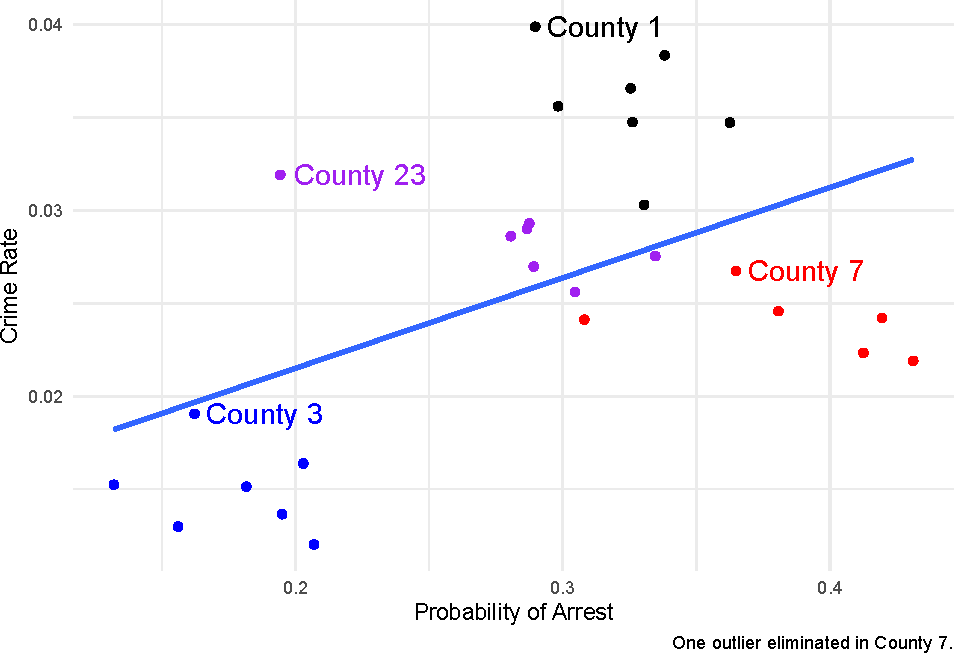
\includegraphics{11-panel-twfe_files/figure-latex/visualize-crime-1.pdf}

\hypertarget{lets-try-the-de-meaning-approach}{%
\subsubsection{Let's try the de-meaning
approach}\label{lets-try-the-de-meaning-approach}}

We can use \texttt{group\_by} to get means-within-groups and subtract
them out.

\begin{Shaded}
\begin{Highlighting}[]
\NormalTok{crime4 }\OtherTok{\textless{}{-}}\NormalTok{ crime4 }\SpecialCharTok{\%\textgreater{}\%}
  \CommentTok{\# Filter to the data points from our graph}
  \FunctionTok{filter}\NormalTok{(county }\SpecialCharTok{\%in\%} \FunctionTok{c}\NormalTok{(}\DecValTok{1}\NormalTok{,}\DecValTok{3}\NormalTok{,}\DecValTok{7}\NormalTok{, }\DecValTok{23}\NormalTok{),}
\NormalTok{         prbarr }\SpecialCharTok{\textless{}}\NormalTok{ .}\DecValTok{5}\NormalTok{) }\SpecialCharTok{\%\textgreater{}\%}
  \FunctionTok{group\_by}\NormalTok{(county) }\SpecialCharTok{\%\textgreater{}\%}
  \FunctionTok{mutate}\NormalTok{(}\AttributeTok{mean\_crime =} \FunctionTok{mean}\NormalTok{(crmrte),}
         \AttributeTok{mean\_prob =} \FunctionTok{mean}\NormalTok{(prbarr)) }\SpecialCharTok{\%\textgreater{}\%}
  \FunctionTok{mutate}\NormalTok{(}\AttributeTok{demeaned\_crime =}\NormalTok{ crmrte }\SpecialCharTok{{-}}\NormalTok{ mean\_crime,}
         \AttributeTok{demeaned\_prob =}\NormalTok{ prbarr }\SpecialCharTok{{-}}\NormalTok{ mean\_prob)}
\end{Highlighting}
\end{Shaded}

\hypertarget{and-regress}{%
\subsubsection{And Regress!}\label{and-regress}}

\begin{Shaded}
\begin{Highlighting}[]
\NormalTok{orig\_data }\OtherTok{\textless{}{-}} \FunctionTok{feols}\NormalTok{(crmrte }\SpecialCharTok{\textasciitilde{}}\NormalTok{ prbarr, }\AttributeTok{data =}\NormalTok{ crime4)}
\NormalTok{de\_mean }\OtherTok{\textless{}{-}} \FunctionTok{feols}\NormalTok{(demeaned\_crime }\SpecialCharTok{\textasciitilde{}}\NormalTok{ demeaned\_prob, }\AttributeTok{data =}\NormalTok{ crime4)}
\FunctionTok{etable}\NormalTok{(orig\_data, de\_mean)}
\end{Highlighting}
\end{Shaded}

\begin{verbatim}
##                         orig_data           de_mean
## Dependent Var.:            crmrte    demeaned_crime
##                                                    
## Constant         0.0118* (0.0050) 1.41e-18 (0.0004)
## prbarr          0.0486** (0.0167)                  
## demeaned_prob                     -0.0305* (0.0117)
## _______________ _________________ _________________
## S.E. type                     IID               IID
## Observations                   27                27
## R2                        0.25308           0.21445
## Adj. R2                   0.22321           0.18303
## ---
## Signif. codes: 0 '***' 0.001 '**' 0.01 '*' 0.05 '.' 0.1 ' ' 1
\end{verbatim}

\hypertarget{interpreting-a-within-relationship}{%
\subsubsection{Interpreting a Within
Relationship}\label{interpreting-a-within-relationship}}

How can we interpret that slope of \texttt{-0.03}? This is all
\emph{within variation} so our interpretation must be
\emph{within-county}. So, ``comparing a county in year A where its
arrest probability is 1 (100 percentage points) higher than it is in
year B, we expect the number of crimes per person to drop by .03.'' Or
if we think we've causally identified it (and want to work on a more
realistic scale), ``raising the arrest probability by 1 percentage point
in a county reduces the number of crimes per person in that county by
.0003''. We're basically ``controlling for county'' (and will do that
explicitly in a moment). So your interpretation should think of it in
that way - \emph{holding county constant} i.e.~\emph{comparing two
observations with the same value of county} i.e.~\emph{comparing a
county to itself at a different point in time}.

\hypertarget{concept-checks}{%
\subsubsection{Concept Checks}\label{concept-checks}}

\begin{itemize}
\tightlist
\item
  Why does subtracting the within-individual mean of each variable
  ``control for individual''?
\item
  In a sentence, interpret the slope coefficient in the estimated model
  \((Y_{it} - \bar{Y}_i) = 2 + 3(X_{it} - \bar{X}_i)\) where \(Y\) is
  ``blood pressure'', \(X\) is ``stress at work'', and \(i\) is an
  individual person
\item
  Is this relationship causal? If not, what assumptions are required for
  it to be causal?
\end{itemize}

\hypertarget{can-we-do-that-all-at-once-yes-with-the-least-squares-dummy-variable-approach}{%
\subsubsection{Can we do that all at once? Yes, with the Least Squares
Dummy Variable
Approach}\label{can-we-do-that-all-at-once-yes-with-the-least-squares-dummy-variable-approach}}

De-meaning takes some steps which could get tedious to write out.
Another way is to include a dummy or category variable for each county.
This is called the Least Squares Dummy Variable approach.

You end up with the same results as if we de-meaned.

\begin{Shaded}
\begin{Highlighting}[]
\NormalTok{lsdv }\OtherTok{\textless{}{-}} \FunctionTok{feols}\NormalTok{(crmrte }\SpecialCharTok{\textasciitilde{}}\NormalTok{ prbarr }\SpecialCharTok{+} \FunctionTok{factor}\NormalTok{(county), }\AttributeTok{data =}\NormalTok{ crime4)}
\FunctionTok{etable}\NormalTok{(orig\_data, de\_mean, lsdv, }\AttributeTok{keep =} \FunctionTok{c}\NormalTok{(}\StringTok{\textquotesingle{}prbarr\textquotesingle{}}\NormalTok{, }\StringTok{\textquotesingle{}demeaned\_prob\textquotesingle{}}\NormalTok{))}
\end{Highlighting}
\end{Shaded}

\begin{verbatim}
##                         orig_data           de_mean              lsdv
## Dependent Var.:            crmrte    demeaned_crime            crmrte
##                                                                      
## prbarr          0.0486** (0.0167)                   -0.0305* (0.0124)
## demeaned_prob                     -0.0305* (0.0117)                  
## _______________ _________________ _________________ _________________
## S.E. type                     IID               IID               IID
## Observations                   27                27                27
## R2                        0.25308           0.21445           0.94114
## Adj. R2                   0.22321           0.18303           0.93044
## ---
## Signif. codes: 0 '***' 0.001 '**' 0.01 '*' 0.05 '.' 0.1 ' ' 1
\end{verbatim}

\hypertarget{why-lsdv}{%
\subsubsection{Why LSDV?}\label{why-lsdv}}

\begin{itemize}
\tightlist
\item
  A benefit of the LSDV approach is that it calculates the fixed effects
  \(\alpha_i\) for you
\item
  We left those out of the table with the \texttt{coefs} argument of
  \texttt{export\_summs} (we rarely want them) but here they are:
\end{itemize}

\begin{Shaded}
\begin{Highlighting}[]
\NormalTok{lsdv}
\end{Highlighting}
\end{Shaded}

\begin{verbatim}
## OLS estimation, Dep. Var.: crmrte
## Observations: 27 
## Standard-errors: IID 
##                   Estimate Std. Error   t value   Pr(>|t|)    
## (Intercept)       0.045631   0.004116  11.08640 1.7906e-10 ***
## prbarr           -0.030491   0.012442  -2.45068 2.2674e-02 *  
## factor(county)3  -0.025308   0.002165 -11.68996 6.5614e-11 ***
## factor(county)7  -0.009870   0.001418  -6.96313 5.4542e-07 ***
## factor(county)23 -0.008587   0.001258  -6.82651 7.3887e-07 ***
## ---
## Signif. codes:  0 '***' 0.001 '**' 0.01 '*' 0.05 '.' 0.1 ' ' 1
## RMSE: 0.001933   Adj. R2: 0.930441
\end{verbatim}

THe interpretation is exactly the same as with a categorical variable -
we have an omitted county, and these show the difference relative to
that omitted county

\hypertarget{why-lsdv-1}{%
\subsubsection{Why LSDV?}\label{why-lsdv-1}}

This also makes clear another element of what's happening! Just like
with a categorical var, the line is moving \emph{up and down} to meet
the counties. Graphically, de-meaning moves all the points together in
the middle to draw a line, while LSDV moves the line up and down to meet
the points

\begin{Shaded}
\begin{Highlighting}[]
\NormalTok{crime4 }\SpecialCharTok{\%\textgreater{}\%}
  \FunctionTok{ungroup}\NormalTok{() }\SpecialCharTok{\%\textgreater{}\%}
  \FunctionTok{mutate}\NormalTok{(}\AttributeTok{pred =} \FunctionTok{predict}\NormalTok{(lsdv)) }\SpecialCharTok{\%\textgreater{}\%}
  \FunctionTok{group\_by}\NormalTok{(county) }\SpecialCharTok{\%\textgreater{}\%}
  \FunctionTok{mutate}\NormalTok{(}\AttributeTok{label =} \FunctionTok{case\_when}\NormalTok{(}
\NormalTok{    crmrte }\SpecialCharTok{==} \FunctionTok{max}\NormalTok{(crmrte) }\SpecialCharTok{\textasciitilde{}} \FunctionTok{paste}\NormalTok{(}\StringTok{\textquotesingle{}County\textquotesingle{}}\NormalTok{,county),}
    \ConstantTok{TRUE} \SpecialCharTok{\textasciitilde{}} \ConstantTok{NA\_character\_}
\NormalTok{  )) }\SpecialCharTok{\%\textgreater{}\%}
  \FunctionTok{ggplot}\NormalTok{(}\FunctionTok{aes}\NormalTok{(}\AttributeTok{x =}\NormalTok{  prbarr, }\AttributeTok{y =}\NormalTok{ crmrte, }\AttributeTok{color =} \FunctionTok{factor}\NormalTok{(county), }\AttributeTok{label =}\NormalTok{ label)) }\SpecialCharTok{+} 
  \FunctionTok{geom\_point}\NormalTok{() }\SpecialCharTok{+} 
  \FunctionTok{geom\_text}\NormalTok{(}\AttributeTok{hjust =} \SpecialCharTok{{-}}\NormalTok{.}\DecValTok{1}\NormalTok{, }\AttributeTok{size =} \DecValTok{14}\SpecialCharTok{/}\NormalTok{.pt) }\SpecialCharTok{+} 
  \FunctionTok{geom\_line}\NormalTok{(}\FunctionTok{aes}\NormalTok{(}\AttributeTok{y =}\NormalTok{ pred, }\AttributeTok{group =}\NormalTok{ county), }\AttributeTok{color =} \StringTok{\textquotesingle{}blue\textquotesingle{}}\NormalTok{) }\SpecialCharTok{+}
  \FunctionTok{labs}\NormalTok{(}\AttributeTok{x =} \StringTok{\textquotesingle{}Probability of Arrest\textquotesingle{}}\NormalTok{, }
       \AttributeTok{y =} \StringTok{\textquotesingle{}Crime Rate\textquotesingle{}}\NormalTok{,}
       \AttributeTok{caption =} \StringTok{\textquotesingle{}One outlier eliminated in County 7.\textquotesingle{}}\NormalTok{) }\SpecialCharTok{+} 
  \CommentTok{\#scale\_x\_continuous(limits = c(.15, 2.5)) + }
  \FunctionTok{guides}\NormalTok{(}\AttributeTok{color =} \ConstantTok{FALSE}\NormalTok{, }\AttributeTok{label =} \ConstantTok{FALSE}\NormalTok{) }\SpecialCharTok{+} 
  \FunctionTok{scale\_color\_manual}\NormalTok{(}\AttributeTok{values =} \FunctionTok{c}\NormalTok{(}\StringTok{\textquotesingle{}black\textquotesingle{}}\NormalTok{,}\StringTok{\textquotesingle{}blue\textquotesingle{}}\NormalTok{,}\StringTok{\textquotesingle{}red\textquotesingle{}}\NormalTok{,}\StringTok{\textquotesingle{}purple\textquotesingle{}}\NormalTok{))}
\end{Highlighting}
\end{Shaded}

\begin{verbatim}
## Warning: The `<scale>` argument of `guides()` cannot be `FALSE`. Use "none" instead as
## of ggplot2 3.3.4.
## This warning is displayed once every 8 hours.
## Call `lifecycle::last_lifecycle_warnings()` to see where this warning was
## generated.
\end{verbatim}

\begin{verbatim}
## Warning: Removed 23 rows containing missing values (`geom_text()`).
\end{verbatim}

\includesvg{11-panel-twfe_files/figure-latex/slopes-1.svg}

\hypertarget{the-pros-dont-use-lsdv}{%
\subsubsection{The ``Pros'' don't use
LSDV}\label{the-pros-dont-use-lsdv}}

Most people do not use LSDB -- it is computationally expensive. If you
get too many fixed effects or too big of data, it just will not wrong.
The professionally-written commands use de-meaning, like
\textbf{fixest}, which is less computationally expensive. See for
yourself!

\begin{Shaded}
\begin{Highlighting}[]
\NormalTok{pro }\OtherTok{\textless{}{-}} \FunctionTok{feols}\NormalTok{(crmrte }\SpecialCharTok{\textasciitilde{}}\NormalTok{ prbarr }\SpecialCharTok{|}\NormalTok{ county, }\AttributeTok{data =}\NormalTok{ crime4)}
\FunctionTok{etable}\NormalTok{(de\_mean, pro)}
\end{Highlighting}
\end{Shaded}

\begin{verbatim}
##                           de_mean               pro
## Dependent Var.:    demeaned_crime            crmrte
##                                                    
## Constant        1.41e-18 (0.0004)                  
## demeaned_prob   -0.0305* (0.0117)                  
## prbarr                            -0.0305* (0.0064)
## Fixed-Effects:  ----------------- -----------------
## county                         No               Yes
## _______________ _________________ _________________
## S.E. type                     IID        by: county
## Observations                   27                27
## R2                        0.21445           0.94114
## Within R2                      --           0.21445
## ---
## Signif. codes: 0 '***' 0.001 '**' 0.01 '*' 0.05 '.' 0.1 ' ' 1
\end{verbatim}

To explain the \textbf{fixest} package, I am borrowing more from Grant
McDermott.

\textbf{\emph{Note}: Grant switches to the starwars dataframe to present
regressions.}

\hypertarget{fixed-effects-with-the-fixest-package}{%
\subsubsection{\texorpdfstring{Fixed effects with the \textbf{fixest}
package}{Fixed effects with the fixest package}}\label{fixed-effects-with-the-fixest-package}}

The simplest (and least efficient) way to include fixed effects in a
regression model is, of course, to use dummy variables. However, it
isn't very efficient or scalable. What's the point learning all that
stuff about the
\href{https://en.wikipedia.org/wiki/Frisch\%E2\%80\%93Waugh\%E2\%80\%93Lovell_theorem}{Frisch-Waugh-Lovell},
within-group transformations, etc. etc. if we can't use them in our
software routines? Again, there are several options to choose from here.
For example, many of you are probably familiar with the excellent
\textbf{lfe} package
(\href{https://cran.r-project.org/web/packages/lfe/index.html}{link}),
which offers near-identical functionality to the popular Stata library,
\textbf{reghdfe} (\href{http://scorreia.com/software/reghdfe/}{link}).
However, for fixed effects models in R, I am going to advocate that you
look no further than the \textbf{fixest} package
(\href{https://lrberge.github.io/fixest}{link}).

\textbf{fixest} is relatively new on the scene and has quickly become
one of my absolute favourite packages. It has an \emph{boatload} of
functionality built in to it: support for nonlinear models,
high-dimensional fixed effects, multiway clustering, multi-model
estimation, LaTeX tables, etc, etc. It is also insanely fast\ldots{} as
in, up to \href{https://lrberge.github.io/fixest/\#benchmarking}{orders
of magnitude} faster than \textbf{lfe} (in R) or \textbf{reghdfe} (in
Stata). I won't be able to cover all of \textbf{fixest}'s features in
depth here --- see the
\href{https://lrberge.github.io/fixest/articles/fixest_walkthrough.html}{introductory
vignette} for a thorough walkthrough --- but I hope to least give you a
sense of why I am so enthusiastic about it. Let's start off with a
simple example before moving on to something slightly more demanding.

\hypertarget{simple-fe-model}{%
\paragraph{Simple FE model}\label{simple-fe-model}}

The package's main function is \texttt{fixest::feols()}, which is used
for estimating linear fixed effects models. The syntax is such that you
first specify the regression model as per normal, and then list the
fixed effect(s) after a \texttt{\textbar{}}. An example may help to
illustrate. Let's say that we again want to run our simple regression of
mass on height, but this time control for species-level fixed
effects.\footnote{Since we specify ``species'' in the fixed effects slot
  below, \texttt{feols()} will automatically coerce it to a factor
  variable even though we didn't explicitly tell it to.}

\begin{Shaded}
\begin{Highlighting}[]
\CommentTok{\# library(fixest) \#\# Already loaded}

\NormalTok{ols\_fe }\OtherTok{=} \FunctionTok{feols}\NormalTok{(mass }\SpecialCharTok{\textasciitilde{}}\NormalTok{ height }\SpecialCharTok{|}\NormalTok{ species, }\AttributeTok{data =}\NormalTok{ starwars) }\DocumentationTok{\#\# Fixed effect(s) go after the "|"}
\NormalTok{ols\_fe}
\end{Highlighting}
\end{Shaded}

\begin{verbatim}
## OLS estimation, Dep. Var.: mass
## Observations: 58 
## Fixed-effects: species: 31
## Standard-errors: Clustered (species) 
##        Estimate Std. Error t value  Pr(>|t|)    
## height 0.974876   0.044291 22.0105 < 2.2e-16 ***
## ---
## Signif. codes:  0 '***' 0.001 '**' 0.01 '*' 0.05 '.' 0.1 ' ' 1
## RMSE: 9.69063     Adj. R2: 0.99282 
##                 Within R2: 0.662493
\end{verbatim}

Note that the resulting model object has automatically clustered the
standard errors by the fixed effect variable (i.e.~species). We'll
explore some more options for adjusting standard errors in
\textbf{fixest} objects shortly. But to preview things, you can specify
the standard errors you want at estimation time\ldots{} or you can
adjust the standard errors for any existing model via
\texttt{summary.fixest()}. For example, here are two equivalent ways to
specify vanilla (iid) standard errors:

\begin{column}{0.48\textwidth}

Specify SEs at estimation time.

\begin{Shaded}
\begin{Highlighting}[]
\FunctionTok{feols}\NormalTok{(mass }\SpecialCharTok{\textasciitilde{}}\NormalTok{ height }\SpecialCharTok{|}\NormalTok{ species, }
      \AttributeTok{data =}\NormalTok{ starwars, }\AttributeTok{se =} \StringTok{\textquotesingle{}standard\textquotesingle{}}\NormalTok{)}
\end{Highlighting}
\end{Shaded}

\begin{verbatim}
## OLS estimation, Dep. Var.: mass
## Observations: 58 
## Fixed-effects: species: 31
## Standard-errors: IID 
##        Estimate Std. Error t value   Pr(>|t|)    
## height 0.974876   0.136463  7.1439 1.3797e-07 ***
## ---
## Signif. codes:  0 '***' 0.001 '**' 0.01 '*' 0.05 '.' 0.1 ' ' 1
## RMSE: 9.69063     Adj. R2: 0.99282 
##                 Within R2: 0.662493
\end{verbatim}

\end{column}

\begin{column}{0.04\textwidth}
~

\end{column}

\begin{column}{0.48\textwidth}

Adjust SEs of an existing model (\texttt{ols\_fe}) on the fly.

\begin{Shaded}
\begin{Highlighting}[]
\FunctionTok{summary}\NormalTok{(ols\_fe, }
        \AttributeTok{se =} \StringTok{\textquotesingle{}standard\textquotesingle{}}\NormalTok{)}
\end{Highlighting}
\end{Shaded}

\begin{verbatim}
## OLS estimation, Dep. Var.: mass
## Observations: 58 
## Fixed-effects: species: 31
## Standard-errors: IID 
##        Estimate Std. Error t value   Pr(>|t|)    
## height 0.974876   0.136463  7.1439 1.3797e-07 ***
## ---
## Signif. codes:  0 '***' 0.001 '**' 0.01 '*' 0.05 '.' 0.1 ' ' 1
## RMSE: 9.69063     Adj. R2: 0.99282 
##                 Within R2: 0.662493
\end{verbatim}

\end{column}

~

Before continuing, let's quickly save a ``tidied'' data frame of the
coefficients for later use. I'll use iid standard errors again, if only
to show you that the \texttt{broom::tidy()} method for \texttt{fixest}
objects also accepts an \texttt{se} argument. This basically just
provides another convenient way for you to adjust standard errors for
your models on the fly.

\begin{Shaded}
\begin{Highlighting}[]
\CommentTok{\# coefs\_fe = tidy(summary(ols\_fe, se = \textquotesingle{}standard\textquotesingle{}), conf.int = TRUE) \#\# same as below}
\NormalTok{coefs\_fe }\OtherTok{=} \FunctionTok{tidy}\NormalTok{(ols\_fe, }\AttributeTok{se =} \StringTok{\textquotesingle{}standard\textquotesingle{}}\NormalTok{, }\AttributeTok{conf.int =} \ConstantTok{TRUE}\NormalTok{)}
\end{Highlighting}
\end{Shaded}

\hypertarget{high-dimensional-fes-and-multiway-clustering}{%
\paragraph{High dimensional FEs and multiway
clustering}\label{high-dimensional-fes-and-multiway-clustering}}

As I already mentioned above, \textbf{fixest} supports (arbitrarily)
high-dimensional fixed effects and (up to fourway) multiway clustering.
To see this in action, let's add ``homeworld'' as an additional fixed
effect to the model.

\begin{Shaded}
\begin{Highlighting}[]
\DocumentationTok{\#\# We now have two fixed effects: species and homeworld}
\NormalTok{ols\_hdfe }\OtherTok{=} \FunctionTok{feols}\NormalTok{(mass }\SpecialCharTok{\textasciitilde{}}\NormalTok{ height }\SpecialCharTok{|}\NormalTok{ species }\SpecialCharTok{+}\NormalTok{ homeworld, }\AttributeTok{data =}\NormalTok{ starwars)}
\NormalTok{ols\_hdfe}
\end{Highlighting}
\end{Shaded}

\begin{verbatim}
## OLS estimation, Dep. Var.: mass
## Observations: 55 
## Fixed-effects: species: 30,  homeworld: 38
## Standard-errors: Clustered (species) 
##        Estimate Std. Error t value Pr(>|t|)    
## height 0.755844   0.332888 2.27057  0.03078 *  
## ---
## Signif. codes:  0 '***' 0.001 '**' 0.01 '*' 0.05 '.' 0.1 ' ' 1
## RMSE: 7.45791     Adj. R2: 1.00768 
##                 Within R2: 0.487231
\end{verbatim}

Easy enough, but the standard errors of the above model are
automatically clustered by species, i.e.~the first fixed effect
variable. Let's go a step further and cluster by both ``species'' and
``homeworld''. \footnote{I make no claims to this is a particularly good
  or sensible clustering strategy, but just go with it.} \textbf{fixest}
provides several ways for us to do this --- via the \texttt{se} or
\texttt{cluster} arguments --- and, again, you can specify your
clustering strategy at estimation time, or adjust the standard errors of
an existing model on-the-fly. I'll (re)assign the model to the same
\texttt{ols\_hdfe} object, but you could, of course, create a new object
if you so wished.

\begin{Shaded}
\begin{Highlighting}[]
\DocumentationTok{\#\# Cluster by both species and homeworld}

\DocumentationTok{\#\# These next few lines all do the same thing. Pick your favourite!}

\DocumentationTok{\#\# Specify desired SEs at estimation time...}
\CommentTok{\# ols\_hdfe = feols(mass \textasciitilde{} height | species + homeworld, se = \textquotesingle{}twoway\textquotesingle{}, data = starwars)}
\CommentTok{\# ols\_hdfe = feols(mass \textasciitilde{} height | species + homeworld, cluster = c(\textquotesingle{}species\textquotesingle{}, \textquotesingle{}homeworld\textquotesingle{}), data = starwars)}
\CommentTok{\# ols\_hdfe = feols(mass \textasciitilde{} height | species + homeworld, cluster = \textasciitilde{} species + homeworld, data = starwars)}
\CommentTok{\# }
\DocumentationTok{\#\#... or, adjust the SEs of an existing model on the fly}
\CommentTok{\# ols\_hdfe = summary(ols\_hdfe, se = \textquotesingle{}twoway\textquotesingle{})}
\CommentTok{\# ols\_hdfe = summary(ols\_hdfe, cluster = c(\textquotesingle{}species\textquotesingle{}, \textquotesingle{}homeworld\textquotesingle{}))}
\NormalTok{ols\_hdfe }\OtherTok{=} \FunctionTok{summary}\NormalTok{(ols\_hdfe, }\AttributeTok{cluster =} \SpecialCharTok{\textasciitilde{}}\NormalTok{ species }\SpecialCharTok{+}\NormalTok{ homeworld) }\DocumentationTok{\#\# I\textquotesingle{}ll go with this one}

\NormalTok{ols\_hdfe}
\end{Highlighting}
\end{Shaded}

\begin{verbatim}
## OLS estimation, Dep. Var.: mass
## Observations: 55 
## Fixed-effects: species: 30,  homeworld: 38
## Standard-errors: Clustered (species & homeworld) 
##        Estimate Std. Error t value   Pr(>|t|)    
## height 0.755844   0.116416 6.49263 4.1625e-07 ***
## ---
## Signif. codes:  0 '***' 0.001 '**' 0.01 '*' 0.05 '.' 0.1 ' ' 1
## RMSE: 7.45791     Adj. R2: 1.00768 
##                 Within R2: 0.487231
\end{verbatim}

\hypertarget{comparing-our-model-coefficients}{%
\paragraph{Comparing our model
coefficients}\label{comparing-our-model-coefficients}}

I want to quickly flag that \textbf{fixest} provides some really nice,
built-in functions for comparing models. For example, you can get
regression tables with
\href{https://lrberge.github.io/fixest/articles/exporting_tables.html}{\texttt{fixest::etable()}}.

\begin{Shaded}
\begin{Highlighting}[]
\FunctionTok{etable}\NormalTok{(ols\_fe, ols\_hdfe)}
\end{Highlighting}
\end{Shaded}

\begin{verbatim}
##                             ols_fe           ols_hdfe
## Dependent Var.:               mass               mass
##                                                      
## height          0.9749*** (0.0443) 0.7558*** (0.1164)
## Fixed-Effects:  ------------------ ------------------
## species                        Yes                Yes
## homeworld                       No                Yes
## _______________ __________________ __________________
## S.E.: Clustered        by: species  by: spec. & home.
## Observations                    58                 55
## R2                         0.99672            0.99815
## Within R2                  0.66249            0.48723
## ---
## Signif. codes: 0 '***' 0.001 '**' 0.01 '*' 0.05 '.' 0.1 ' ' 1
\end{verbatim}

Similarly, the
\href{https://lrberge.github.io/fixest/reference/coefplot.html}{\texttt{fixest::coefplot()}}
function for plotting estimation results:

\begin{Shaded}
\begin{Highlighting}[]
\FunctionTok{coefplot}\NormalTok{(}\FunctionTok{list}\NormalTok{(ols\_fe, ols\_hdfe))}

\DocumentationTok{\#\# Add legend (optional)}
\FunctionTok{legend}\NormalTok{(}\StringTok{"bottomleft"}\NormalTok{, }\AttributeTok{col =} \DecValTok{1}\SpecialCharTok{:}\DecValTok{2}\NormalTok{, }\AttributeTok{lwd =} \DecValTok{1}\NormalTok{, }\AttributeTok{pch =} \FunctionTok{c}\NormalTok{(}\DecValTok{20}\NormalTok{, }\DecValTok{17}\NormalTok{),}
       \AttributeTok{legend =} \FunctionTok{c}\NormalTok{(}\StringTok{"FE and no clustering"}\NormalTok{, }\StringTok{"HDFE and twoway clustering"}\NormalTok{))}
\end{Highlighting}
\end{Shaded}

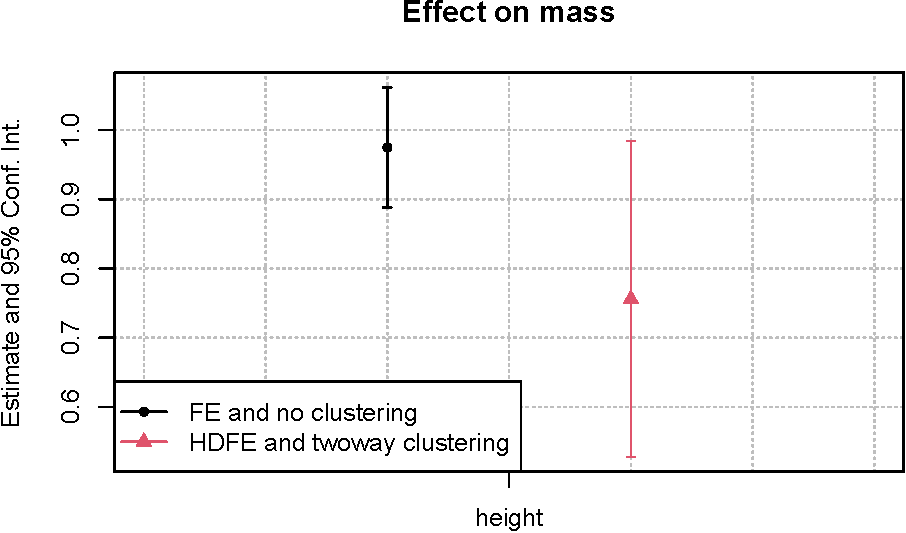
\includegraphics{11-panel-twfe_files/figure-latex/coefplot-1.pdf}

\texttt{coefplot()} is especially useful for tracing the evolution of
treatment effects over time, as in a difference-in-differences setup
(see
\href{https://lrberge.github.io/fixest/reference/coefplot.html\#examples}{Examples}).
However, I realise some people may find it a bit off-putting that it
produces base R plots, rather than a \textbf{ggplot2} object. We'll get
to an automated \textbf{ggplot2} coefficient plot solution further below
with \texttt{modelsummary::modelplot()}. Nevertheless, let me close this
out this section by demonstrating the relative ease with which you can
do this ``manually''. Consider the below example, which leverages the
fact that we have saved (or can save) regression models as data frames
with \texttt{broom::tidy()}. As I suggested earlier, this makes it
simple to construct our own bespoke coefficient plots.

\begin{Shaded}
\begin{Highlighting}[]
\CommentTok{\# library(ggplot2) \#\# Already loaded}

\DocumentationTok{\#\# First get tidied output of the ols\_hdfe object}
\NormalTok{coefs\_hdfe }\OtherTok{=} \FunctionTok{tidy}\NormalTok{(ols\_hdfe, }\AttributeTok{conf.int =} \ConstantTok{TRUE}\NormalTok{)}

\FunctionTok{bind\_rows}\NormalTok{(}
\NormalTok{  coefs\_fe }\SpecialCharTok{\%\textgreater{}\%} \FunctionTok{mutate}\NormalTok{(}\AttributeTok{reg =} \StringTok{"Model 1}\SpecialCharTok{\textbackslash{}n}\StringTok{FE and no clustering"}\NormalTok{),}
\NormalTok{  coefs\_hdfe }\SpecialCharTok{\%\textgreater{}\%} \FunctionTok{mutate}\NormalTok{(}\AttributeTok{reg =} \StringTok{"Model 2}\SpecialCharTok{\textbackslash{}n}\StringTok{HDFE and twoway clustering"}\NormalTok{)}
\NormalTok{  ) }\SpecialCharTok{\%\textgreater{}\%}
  \FunctionTok{ggplot}\NormalTok{(}\FunctionTok{aes}\NormalTok{(}\AttributeTok{x=}\NormalTok{reg, }\AttributeTok{y=}\NormalTok{estimate, }\AttributeTok{ymin=}\NormalTok{conf.low, }\AttributeTok{ymax=}\NormalTok{conf.high)) }\SpecialCharTok{+}
  \FunctionTok{geom\_pointrange}\NormalTok{() }\SpecialCharTok{+}
  \FunctionTok{labs}\NormalTok{(}\AttributeTok{Title =} \StringTok{"Marginal effect of height on mass"}\NormalTok{) }\SpecialCharTok{+}
  \FunctionTok{geom\_hline}\NormalTok{(}\AttributeTok{yintercept =} \DecValTok{0}\NormalTok{, }\AttributeTok{col =} \StringTok{"orange"}\NormalTok{) }\SpecialCharTok{+}
  \FunctionTok{ylim}\NormalTok{(}\SpecialCharTok{{-}}\FloatTok{0.5}\NormalTok{, }\ConstantTok{NA}\NormalTok{) }\SpecialCharTok{+} \DocumentationTok{\#\# Added a bit more bottom space to emphasize the zero line}
  \FunctionTok{labs}\NormalTok{(}
    \AttributeTok{title =} \StringTok{"\textquotesingle{}Effect\textquotesingle{} of height on mass"}\NormalTok{,}
    \AttributeTok{caption =} \StringTok{"Data: Characters from the Star Wars universe"}
\NormalTok{    ) }\SpecialCharTok{+}
  \FunctionTok{theme}\NormalTok{(}\AttributeTok{axis.title.x =} \FunctionTok{element\_blank}\NormalTok{())}
\end{Highlighting}
\end{Shaded}

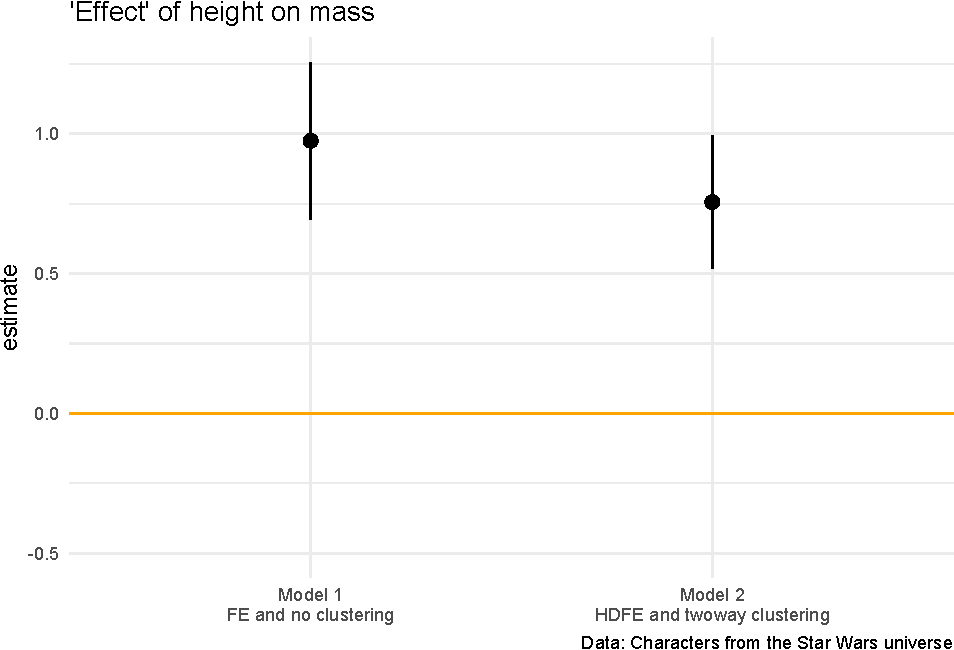
\includegraphics{11-panel-twfe_files/figure-latex/fe_mods_compared-1.pdf}

FWIW, we'd normally expect our standard errors to blow up with
clustering. Here that effect appears to be outweighed by the increased
precision brought on by additional fixed effects. Still, I wouldn't put
too much thought into it. Our clustering choice doesn't make much sense
and I really just trying to demonstrate the package syntax.

\hypertarget{aside-on-standard-errors}{%
\paragraph{Aside on standard errors}\label{aside-on-standard-errors}}

We've now seen the various options that \textbf{fixest} has for
specifying different standard error structures. In short, you invoke
either of the \texttt{se} or \texttt{cluster} arguments. Moreover, you
can choose to do so either at estimation time, or by adjusting the
standard errors for an existing model post-estimation (e.g.~with
\texttt{summary.fixest(mod,\ cluster\ =\ ...)}). There are two
additional points that I want to draw your attention to.

First, if you're coming from another statistical language, adjusting the
standard errors post-estimation (rather than always at estimation time)
may seem slightly odd. But this behaviour is actually extremely
powerful, because it allows us to analyse the effect of different error
structures \emph{on-the-fly} without having to rerun the entire model
again. \textbf{fixest} is already the fastest game in town, but just
think about the implied time savings for really large models.\footnote{To
  be clear, adjusting the standard errors via, say,
  \texttt{summary.fixest()} completes instantaneously.} I'm a huge fan
of the flexibility, safety, and speed that on-the-fly standard error
adjustment offers us. I even wrote a whole
\href{https://grantmcdermott.com/better-way-adjust-SEs/}{blog post}
about it if you'd like to read more.

Second, reconciling standard errors across different software is a much
more complicated process than you may realise. There are a number of
unresolved theoretical issues to consider --- especially when it comes
to multiway clustering --- and package maintainers have to make a number
of arbitrary decisions about the best way to account for these. See
\href{https://github.com/sgaure/lfe/issues/1\#issuecomment-530643808}{here}
for a detailed discussion. Luckily, Laurent (the \textbf{fixest} package
author) has taken the time to write out a
\href{https://lrberge.github.io/fixest/articles/standard_errors.html}{detailed
vignette} about how to replicate standard errors from other methods and
software packages.\footnote{If you want a deep dive into the theory with
  even more simulations, then
  \href{http://sandwich.r-forge.r-project.org/articles/jss_2020.html}{this
  paper} by the authors of the \textbf{sandwich} paper is another
  excellent resource.}

\hypertarget{presentation}{%
\subsection{Presentation}\label{presentation}}

\hypertarget{figures}{%
\subsubsection{Figures}\label{figures}}

\hypertarget{coefficient-plots}{%
\paragraph{Coefficient plots}\label{coefficient-plots}}

We've already worked through an example of how to extract and compare
model coefficients
\protect\hyperlink{comparing-our-model-coefficients}{here}. I use this
``manual'' approach to visualizing coefficient estimates all the time.
However, our focus on \textbf{modelsummary} in the preceding section
provides a nice segue to another one of the package's features:
\href{https://vincentarelbundock.github.io/modelsummary/articles/modelplot.html}{\texttt{modelplot()}}.
Consider the following, which shows both the degree to which
\texttt{modelplot()} automates everything and the fact that it readily
accepts regular \textbf{ggplot2} syntax.

\begin{Shaded}
\begin{Highlighting}[]
\CommentTok{\# library(modelsummary) \#\# Already loaded}
\NormalTok{mods }\OtherTok{=} \FunctionTok{list}\NormalTok{(}\StringTok{\textquotesingle{}FE, no clustering\textquotesingle{}} \OtherTok{=} \FunctionTok{summary}\NormalTok{(ols\_fe, }\AttributeTok{se =} \StringTok{\textquotesingle{}standard\textquotesingle{}}\NormalTok{))}

\FunctionTok{modelplot}\NormalTok{(mods) }\SpecialCharTok{+}
  \DocumentationTok{\#\# You can further modify with normal ggplot2 commands...}
  \FunctionTok{coord\_flip}\NormalTok{() }\SpecialCharTok{+} 
  \FunctionTok{labs}\NormalTok{(}
    \AttributeTok{title =} \StringTok{"\textquotesingle{}Effect\textquotesingle{} of height on mass"}\NormalTok{,}
    \AttributeTok{subtitle =} \StringTok{"Comparing fixed effect models"}
\NormalTok{    )}
\end{Highlighting}
\end{Shaded}

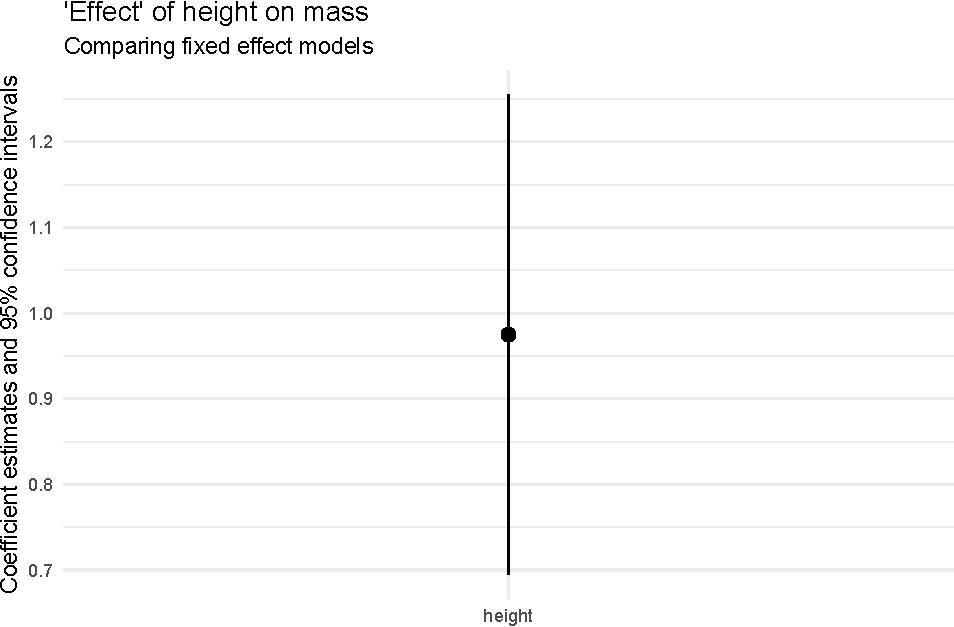
\includegraphics{11-panel-twfe_files/figure-latex/modplot-1.pdf}

\hypertarget{difference-in-differences}{%
\subsection{Difference-in-differences}\label{difference-in-differences}}

One of the most popular uses of fixed effects is to implement
difference-in-difference designs. I vusalize how that works for you
below.

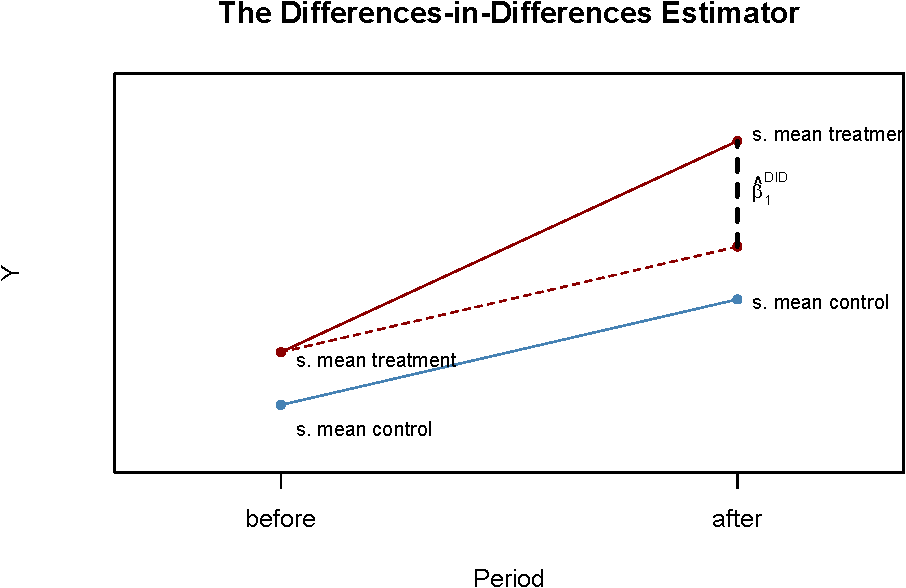
\includegraphics{11-panel-twfe_files/figure-latex/did-1.pdf}

\hypertarget{diff-in-diff-with-data}{%
\subsubsection{Diff-in-diff with data}\label{diff-in-diff-with-data}}

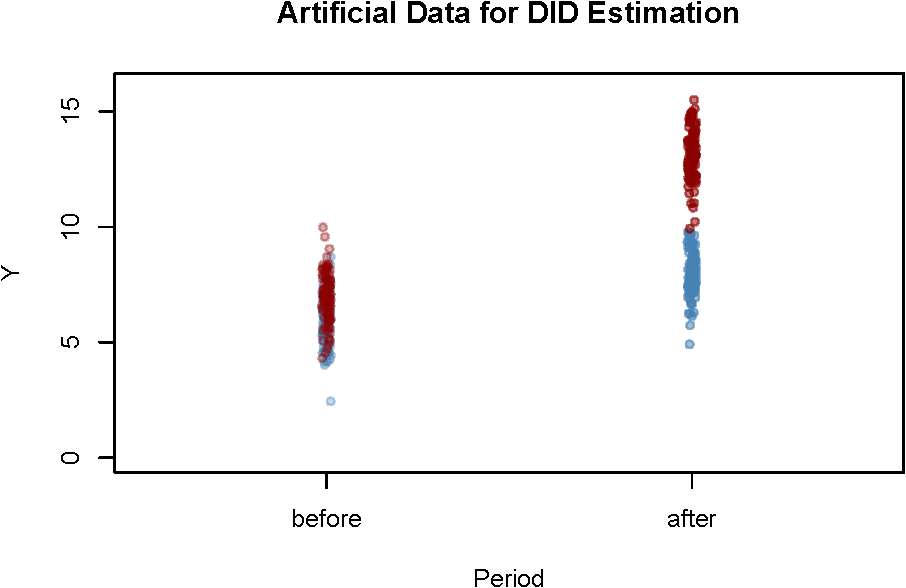
\includegraphics{11-panel-twfe_files/figure-latex/did-data-1.pdf}

\hypertarget{instrumental-variables}{%
\subsection{Instrumental variables}\label{instrumental-variables}}

As you would have guessed by now, there are a number of ways to run
instrumental variable (IV) regressions in R. I'll walk through three
different options using the \texttt{ivreg::ivreg()},
\texttt{estimatr::iv\_robust()}, and \texttt{fixest::feols()} functions,
respectively. These are all going to follow a similar syntax, where the
IV first-stage regression is specified in a multi-part formula
(i.e.~where formula parts are separated by one or more pipes,
\textbf{\texttt{\textbar{}}}). However, there are also some subtle and
important differences, which is why I want to go through each of them.
After that, I'll let you decide which of the three options is your
favourite.

The dataset that we'll be using for this section describes cigarette
demand for the 48 continental US states in 1995, and is taken from the
\textbf{ivreg} package. Here's a quick a peek:

\begin{Shaded}
\begin{Highlighting}[]
\FunctionTok{data}\NormalTok{(}\StringTok{"CigaretteDemand"}\NormalTok{, }\AttributeTok{package =} \StringTok{"ivreg"}\NormalTok{)}
\FunctionTok{head}\NormalTok{(CigaretteDemand)}
\end{Highlighting}
\end{Shaded}

\begin{verbatim}
##        packs   rprice  rincome  salestax   cigtax  packsdiff  pricediff
## AL 101.08543 103.9182 12.91535 0.9216975 26.57481 -0.1418075 0.09010222
## AR 111.04297 115.1854 12.16907 5.4850193 36.41732 -0.1462808 0.19998082
## AZ  71.95417 130.3199 13.53964 6.2057067 42.86964 -0.3733741 0.25576681
## CA  56.85931 138.1264 16.07359 9.0363074 40.02625 -0.5682141 0.32079587
## CO  82.58292 109.8097 16.31556 0.0000000 28.87139 -0.3132622 0.22587189
## CT  79.47219 143.2287 20.96236 8.1072834 48.55643 -0.3184911 0.18546746
##    incomediff salestaxdiff  cigtaxdiff
## AL 0.18222144    0.1332853 -3.62965832
## AR 0.15055894    5.4850193  2.03070663
## AZ 0.05379983    1.4004856 14.05923036
## CA 0.02266877    3.3634447 15.86267924
## CO 0.13002974    0.0000000  0.06098283
## CT 0.18404197   -0.7062239  9.52297455
\end{verbatim}

Now, assume that we are interested in regressing the number of
cigarettes packs consumed per capita on their average price and people's
real incomes. The problem is that the price is endogenous, because it is
simultaneously determined by demand and supply. So we need to instrument
for it using cigarette sales tax. That is, we want to run the following
two-stage IV regression.

\[Price_i = \pi_0 + \pi_1 SalesTax_i + v_i  \hspace{1cm} \text{(First stage)}\]
\[Packs_i = \beta_0 + \beta_2\widehat{Price_i} + \beta_1 RealIncome_i + u_i \hspace{1cm} \text{(Second stage)}\]

\hypertarget{iv-with-fixestfeols}{%
\subsubsection{\texorpdfstring{IV with
\texttt{fixest::feols()}}{IV with fixest::feols()}}\label{iv-with-fixestfeols}}

Finally, we get back to the \texttt{fixest::feols()} function that we've
already seen above. Truth be told, this is the IV option that I use most
often in my own work. In part, this statement reflects the fact that I
work mostly with panel data and will invariably be using \textbf{fixest}
anyway. But I also happen to like its IV syntax a lot. The key thing is
to specify the IV first-stage as a separate formula in the \emph{final}
slot of the model call.\footnote{This closely resembles
  \href{https://www.stata.com/manuals13/rivregress.pdf}{Stata's
  approach} to writing out the IV first-stage, where you specify the
  endogenous variable(s) and the instruments together in a slot.} For
example, if we had \texttt{fe} fixed effects, then the model call would
be
\texttt{y\ \textasciitilde{}\ ex\ \textbar{}\ fe\ \textbar{}\ en\ \textasciitilde{}\ in}.
Since we don't have any fixed effects in our current cigarette demand
example, the first-stage will come directly after the exogenous
variables:

\begin{Shaded}
\begin{Highlighting}[]
\CommentTok{\# library(fixest) \#\# Already loaded}

\NormalTok{iv\_feols }\OtherTok{=} 
  \FunctionTok{feols}\NormalTok{(}
    \FunctionTok{log}\NormalTok{(packs) }\SpecialCharTok{\textasciitilde{}} \FunctionTok{log}\NormalTok{(rincome) }\SpecialCharTok{|} \DocumentationTok{\#\# y \textasciitilde{} ex}
      \FunctionTok{log}\NormalTok{(rprice) }\SpecialCharTok{\textasciitilde{}}\NormalTok{ salestax,   }\DocumentationTok{\#\# en \textasciitilde{} in (IV first{-}stage; must be the final slot)}
    \AttributeTok{data =}\NormalTok{ CigaretteDemand}
\NormalTok{    )}
\CommentTok{\# summary(iv\_feols, stage = 1) \#\# Show the 1st stage in detail}
\NormalTok{iv\_feols}
\end{Highlighting}
\end{Shaded}

\begin{verbatim}
## TSLS estimation, Dep. Var.: log(packs), Endo.: log(rprice), Instr.: salestax
## Second stage: Dep. Var.: log(packs)
## Observations: 48 
## Standard-errors: IID 
##                  Estimate Std. Error   t value   Pr(>|t|)    
## (Intercept)      9.430658   1.358366  6.942648 1.2395e-08 ***
## fit_log(rprice) -1.143375   0.359486 -3.180583 2.6617e-03 ** 
## log(rincome)     0.214515   0.268585  0.798687 4.2867e-01    
## ---
## Signif. codes:  0 '***' 0.001 '**' 0.01 '*' 0.05 '.' 0.1 ' ' 1
## RMSE: 0.183555   Adj. R2: 0.393109
## F-test (1st stage), log(rprice): stat = 45.2  , p = 2.655e-8, on 1 and 45 DoF.
##                      Wu-Hausman: stat =  1.102, p = 0.299559, on 1 and 44 DoF.
\end{verbatim}

Again, I emphasise that the IV first-stage must always come last in the
\texttt{feols()} model call. Just to be pedantic --- but also to
demonstrate how easy \textbf{fixest}'s IV functionality extends to panel
settings --- here's a final \texttt{feols()} example. This time, I'll
use a panel version of the same US cigarette demand data that includes
entries from both 1985 and 1995. The dataset originally comes from the
\textbf{AER} package, but we can download it from the web as follows.
Note that I'm going to modify some variables to make it better
comparable to our previous examples.

\begin{Shaded}
\begin{Highlighting}[]
\DocumentationTok{\#\# Get the data}
\NormalTok{url }\OtherTok{=} \StringTok{\textquotesingle{}https://vincentarelbundock.github.io/Rdatasets/csv/AER/CigarettesSW.csv\textquotesingle{}} 
\NormalTok{cigs\_panel }\OtherTok{=}
  \FunctionTok{read.csv}\NormalTok{(url, }\AttributeTok{row.names =} \DecValTok{1}\NormalTok{) }\SpecialCharTok{\%\textgreater{}\%}
  \FunctionTok{mutate}\NormalTok{(}
    \AttributeTok{rprice =}\NormalTok{ price}\SpecialCharTok{/}\NormalTok{cpi,}
    \AttributeTok{rincome =}\NormalTok{ income}\SpecialCharTok{/}\NormalTok{population}\SpecialCharTok{/}\NormalTok{cpi}
\NormalTok{    )}
\FunctionTok{head}\NormalTok{(cigs\_panel)}
\end{Highlighting}
\end{Shaded}

\begin{verbatim}
##   state year   cpi population    packs    income  tax     price     taxs
## 1    AL 1985 1.076    3973000 116.4863  46014968 32.5 102.18167 33.34834
## 2    AR 1985 1.076    2327000 128.5346  26210736 37.0 101.47500 37.00000
## 3    AZ 1985 1.076    3184000 104.5226  43956936 31.0 108.57875 36.17042
## 4    CA 1985 1.076   26444000 100.3630 447102816 26.0 107.83734 32.10400
## 5    CO 1985 1.076    3209000 112.9635  49466672 31.0  94.26666 31.00000
## 6    CT 1985 1.076    3201000 109.2784  60063368 42.0 128.02499 51.48333
##      rprice  rincome
## 1  94.96438 10.76387
## 2  94.30762 10.46817
## 3 100.90962 12.83046
## 4 100.22058 15.71332
## 5  87.60842 14.32619
## 6 118.98234 17.43861
\end{verbatim}

Let's run a panel IV now, where we'll explicitly account for year and
state fixed effects.

\begin{Shaded}
\begin{Highlighting}[]
\NormalTok{iv\_feols\_panel }\OtherTok{=} 
  \FunctionTok{feols}\NormalTok{(}
    \FunctionTok{log}\NormalTok{(packs) }\SpecialCharTok{\textasciitilde{}} \FunctionTok{log}\NormalTok{(rincome) }\SpecialCharTok{|} 
\NormalTok{      year }\SpecialCharTok{+}\NormalTok{ state }\SpecialCharTok{|}            \DocumentationTok{\#\# Now include FEs slot}
      \FunctionTok{log}\NormalTok{(rprice) }\SpecialCharTok{\textasciitilde{}}\NormalTok{ taxs,       }\DocumentationTok{\#\# IV first{-}stage still comes last}
    \AttributeTok{data =}\NormalTok{ cigs\_panel}
\NormalTok{  )}
\CommentTok{\# summary(iv\_feols\_panel, stage = 1) \#\# Show the 1st stage in detail}
\NormalTok{iv\_feols\_panel}
\end{Highlighting}
\end{Shaded}

\begin{verbatim}
## TSLS estimation, Dep. Var.: log(packs), Endo.: log(rprice), Instr.: taxs
## Second stage: Dep. Var.: log(packs)
## Observations: 96 
## Fixed-effects: year: 2,  state: 48
## Standard-errors: Clustered (year) 
##                  Estimate Std. Error       t value   Pr(>|t|)    
## fit_log(rprice) -1.279349   2.11e-15 -6.071802e+14 1.0485e-15 ***
## log(rincome)     0.443422   1.41e-15  3.138717e+14 2.0283e-15 ***
## ---
## Signif. codes:  0 '***' 0.001 '**' 0.01 '*' 0.05 '.' 0.1 ' ' 1
## RMSE: 0.044789     Adj. R2: 0.92791 
##                  Within R2: 0.533965
## F-test (1st stage), log(rprice): stat = 111.0    , p = 7.535e-14, on 1 and 46 DoF.
##                      Wu-Hausman: stat =   6.02154, p = 0.018161 , on 1 and 44 DoF.
\end{verbatim}

Good news, our coefficients are around the same magnitude. But the
increased precision of the panel model has yielded gains in statistical
significance.

\hypertarget{further-resources}{%
\subsection{Further resources}\label{further-resources}}

\begin{itemize}
\tightlist
\item
  \href{https://twitter.com/edrubin}{Ed Rubin} has outstanding
  \href{http://edrub.in/teaching.html}{teaching notes} for econometrics
  with R on his website. This includes both
  \href{https://github.com/edrubin/EC421S19}{undergrad-} and
  \href{https://github.com/edrubin/EC525S19}{graduate-}level courses.
  Seriously, check them out.
\item
  Several introductory texts are freely available, including
  \href{https://www.econometrics-with-r.org/}{\emph{Introduction to
  Econometrics with R}} (Christoph Hanck \emph{et al.}),
  \href{http://www.urfie.net/}{\emph{Using R for Introductory
  Econometrics}} (Florian Heiss), and
  \href{https://moderndive.com/}{\emph{Modern Dive}} (Chester Ismay and
  Albert Kim).
\item
  \href{https://twitter.com/tyleransom}{Tyler Ransom} has a nice
  \href{https://github.com/tyleransom/EconometricsLabs/blob/master/tidyRcheatsheet.pdf}{cheat
  sheet} for common regression tasks and specifications.
\item
  \href{https://twitter.com/itamarcaspi}{Itamar Caspi} has written a
  neat unofficial appendix to this lecture,
  \href{https://itamarcaspi.rbind.io/post/recipes-for-dummies/}{\emph{recipes
  for Dummies}}. The title might be a little inscrutable if you haven't
  heard of the \texttt{recipes} package before, but basically it handles
  ``tidy'' data preprocessing, which is an especially important topic
  for machine learning methods. We'll get to that later in course, but
  check out Itamar's post for a good introduction.
\item
  I promised to provide some links to time series analysis. The good
  news is that R's support for time series is very, very good. The
  \href{https://cran.r-project.org/web/views/TimeSeries.html}{Time
  Series Analysis} task view on CRAN offers an excellent overview of
  available packages and their functionality.
\item
  Lastly, for more on visualizing regression output, I highly encourage
  you to look over Chapter 6 of Kieran Healy's
  \href{https://socviz.co/modeling.html}{\emph{Data Visualization: A
  Practical Guide}}. Not only will learn how to produce beautiful and
  effective model visualizations, but you'll also pick up a variety of
  technical tips.
\end{itemize}

\end{document}
